\documentclass[english, a4paper, oneside, onecolumn, openany,article]{memoir}
\usepackage{fix-cm,fixltx2e}
\usepackage{babel}  % babel: Hyphenation patterns and language specific strings
\usepackage{varioref}
\usepackage[colorlinks,linkcolor=black,urlcolor=black,citecolor=black]{hyperref}
\usepackage[colorinlistoftodos]{todonotes}
\usepackage[latin1]{inputenc}
\usepackage{graphicx}
\usepackage{listings}
\usepackage[square,numbers]{natbib}
\usepackage{url}
\usepackage{pslatex}
\usepackage{multirow}
\usepackage[T1]{fontenc}
\usepackage{eso-pic}
\usepackage{xcolor,calc}
\usepackage{pdfpages}
\newsubfloat{figure}
\usepackage{placeins} % gives me FloatBarrier
%Forhindrer floats i at flyde ind i næste afsnit
\let\oldsection=\section % gemmer den gamle definition
\renewcommand\section{\FloatBarrier\oldsection}

\makeatletter
\renewcommand\fps@figure{htbp} % Force figure placement
\renewcommand\fps@table{htbp}
\makeatother

% setup captions
\hangcaption
\changecaptionwidth
\captionwidth{9cm}


\title{Advanced Data Management - Assignment 1\\Value of Serializability}
\author{S\o ren Bjerregaard Vrist - 151082-sbvr@itu.dk\\ \\Undervisere: Philippe Bonnet - phbo@itu.dk og
Rasmus Pagh - pagh@itu.dk\\ITU Copenhagen}

\begin{document}
\maketitle
\newpage

This is the solution and logbog book of S\o ren B. Vrist comprising a description of the execution
of experiments as well as results and a discussion of what the experiments show
and why.

The assignment states two questions to be answered. Question one is about
reponse time vs. correctness of different isolationlevels and concurrency
levels and results and discussion is placed in Section \ref{sec:illcorr}.
Question two is about ``currently commited semantics'' of DB2 and the results of
the experiment and a discussion of these is included in Section
\ref{sec:curcommit}.\\

The assignment provides a script which supposedly executes a number of updates
on a table while doing a aggregate query covering all rows in the table. 
The table is initialized with 1000000 rows via the ``gentable'' script also
provided in the assignment zip.\\

The execution of the experiments showed some lackings in the provided script and
section \ref{sec:add} contains my additonal experiments with a changed script.

\chapter{Illustration of correctness}\label{sec:illcorr}
This section will first provide the description of doing the experiment with
provided scripts. We are trying to show that the tradeoff for serializable
transactions is throughput/performance vs. correctness.


\section{Results}
Based on the given \verb|run.py| I graphed two graphs. Figure
\ref{fig:origtime} and \ref{fig:origcorrect} is based on the output of
\verb|run.py|. We are trying to show that with ``restrictive'' isolation levels
- nearing on complete serialized with Repeatable read - you sacrifice
performance but gain correctness.
\begin{figure}
  \centering
  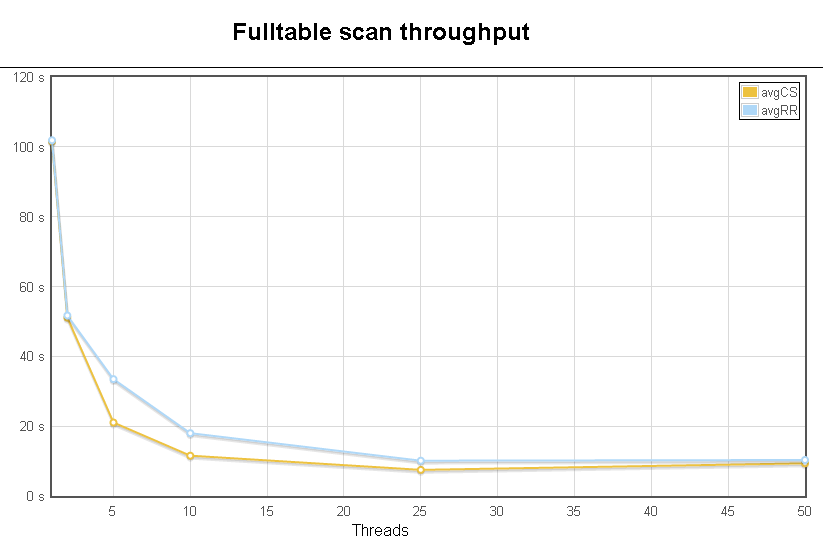
\includegraphics[width=12cm]{assignment1/origtime}
  \caption[Average time over 5 runs]{Average time over 5 runs as a function of
  swap-threads for both Cursor Stability(CS) and Repeatable Read(RR) isolation levels.\\
  We would expect to non-neglible difference between CS and RR but to me it is
  not conclusive in this graph. The runtime is improved on increased parallelism
  for both isolation levels}\label{fig:origtime}
\end{figure}

Figure \ref{fig:origtime} shows the average runtime(y-axis) for 5 runs by run.py for
each level of concurrency (x-axis).

\begin{figure}
  \center:ing
  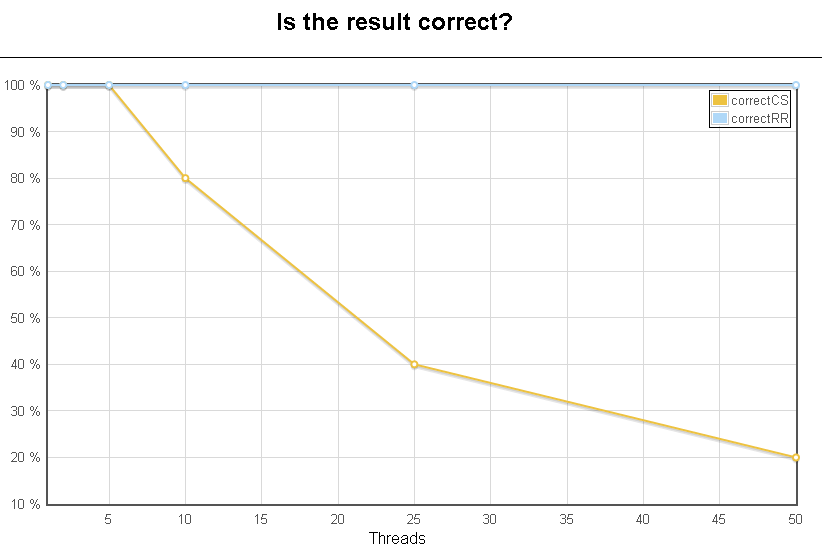
\includegraphics[width=12cm]{assignment1/origcorrect}
  \caption{Average time over 5 runs as a function of swap-threads.}\label{fig:origcorrect}
\end{figure}

\section{Additional experiment}\label{sec:add}
As mentioned previously, I modified the given run.py to perform another kind of
experiment. \\

The basic experiment is layed out as so:
\begin{itemize}
   \item Do $N$ sums spread over $T$ threads
   \item Do $N$ swaps on each thread with $T$ threads, sleep $S$ seconds between each swap.
   \item When all sums are done, terminate the process and the remaining swap
     threads.
\end{itemize}
The idea is to ensure that swaps are happening ``all the time'' while the sums
are being performed - The sums are the ``thing'' we are measuring. Several sums
are performed to be sure that they will be influenced by the swaps. The timings
are normalized by the number of sums performed giving a throughput with the unit
of ``Sum/s''. Figure \ref{fig:curontp} shows the result of this script. This
shows that the throughput:
\begin{enumerate}
  \item is not improved by concurrency for CS isolation level - and 
  \item is somewhat hampered by concurrency for RR isolation.
\end{enumerate}
The first explantion of 1) is that the throughput is at a limit somewhere else,
even with only one thread. 2) fits with the serializable isolation level. More
locking work needs to be done when concurrency is high.

\begin{figure}
  \centering
  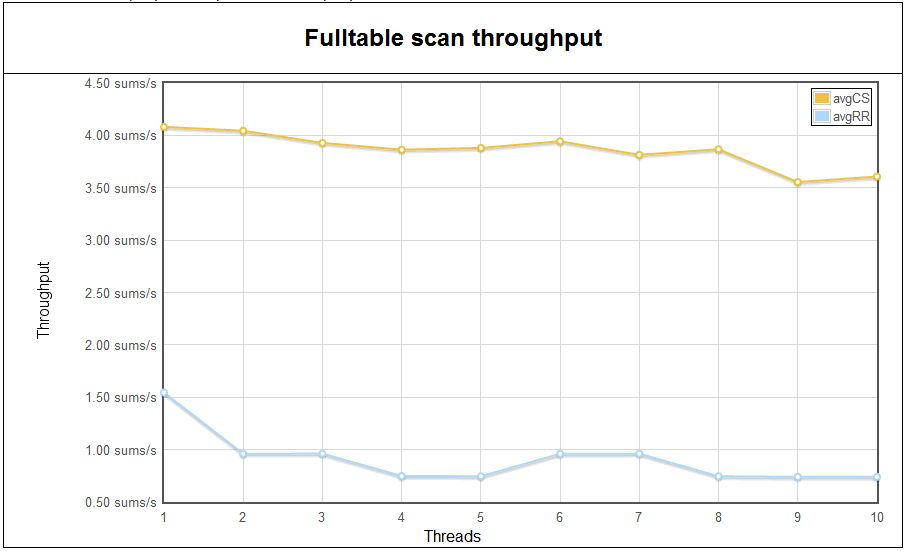
\includegraphics[width=12cm]{assignment1/curon_tp}
  \caption[Average time over 5 runs - new script]{Average time over 5 runs as a function of
  swap-threads for both Cursor Stability(CS) and Repeatable Read(RR) isolation levels.\\
  No improvements with higher concurrency}\label{fig:curontp}
\end{figure}

\begin{figure}
  \centering
  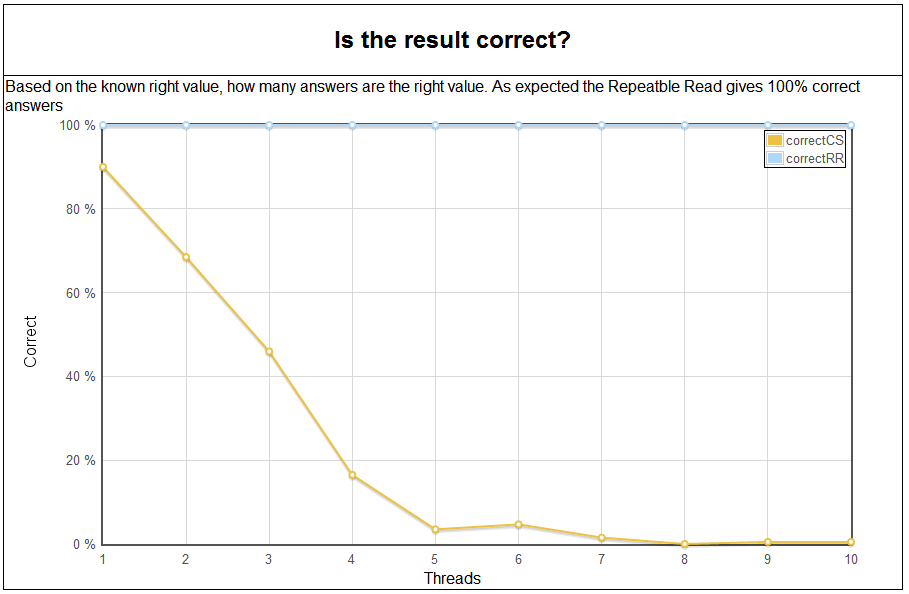
\includegraphics[width=12cm]{assignment1/curon_corr}
  \caption[Correctness - new script]{Correctness as a function of
  swap-threads for both Cursor Stability(CS) and Repeatable Read(RR) isolation
  levels.\\ Same correctness view as the orignal script }\label{fig:curoncorr}
\end{figure}

\section{Conclusion}
The experiements support the thesis that dirty reads allows for higher
throughput but sacrificing correctness as illustrated in the graphs for both
experiments.


\chapter{Currently Committed}\label{sec:curcommit}
When experimenting with currently\_commited semantics, I wasn't able to spot any
difference when using the original script(which supports my thesis that the
original script doesnt measure performance data of the database but only the
python time.sleep method). When using my own script from Section
\ref{sec:add} some difference can be seen. \\

Currently Commited semantics allows the DB2 engine (during CS isolation) to not
wait on row looks when reading. By always using whatever is already committed
when trying to read a row that is locked no wait is neccesary. As the
isolation level already allows dirty reads, this is still ``valid'' data. This
should speed up CS queries under high concurrency.

\section{Results}
Figure \ref{fig:curofftp} show the graph for the same experiment with currently
commited semantics off. Notice that the general throughput (for thread > 1) is
lower than in the same graph above (Figure \ref{fig:curontp} - the default
behavior in DB 9.7 is with Currently Commited semantics ON).

\begin{figure}
  \centering
  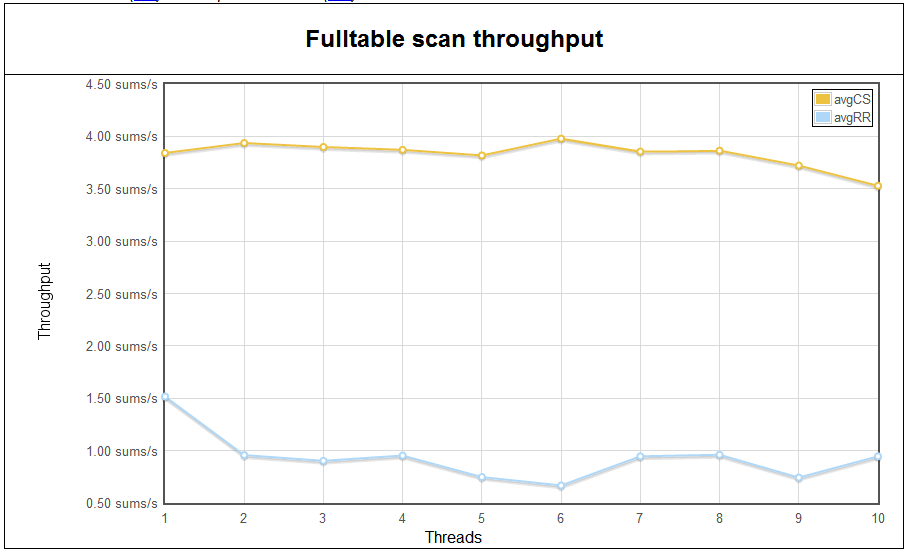
\includegraphics[width=12cm]{assignment1/curoff_tp}
  \caption[Average time over 5 runs - new script, currently commited semantics
  off]{Average time over 5 runs as a function of
  swap-threads for both Cursor Stability(CS) and Repeatable Read(RR) isolation
  levels with currently committed semantics OFF.\\
  Just a tiny bit lower throughput than the same graph with currently commited
  semantics on(Figure \ref{fig:curontp})}\label{fig:curofftp}
\end{figure}

I see no noticable difference in the correctness graph (Figure
\ref{fig:curoffcorr}).

\begin{figure}
  \centering
  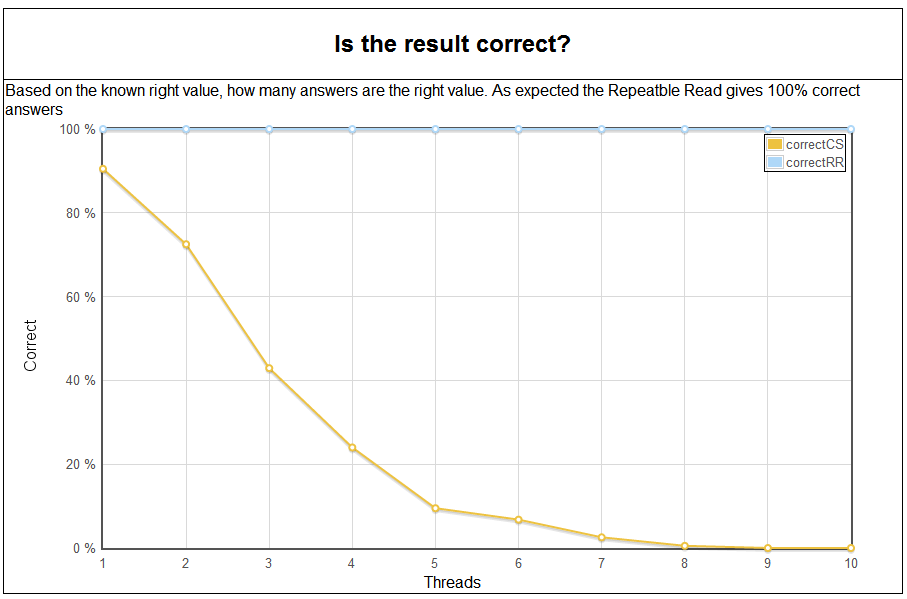
\includegraphics[width=12cm]{assignment1/curoff_corr}
  \caption[Correctness - new script,currently commited semantics off
  ]{Correctness as a function of
  swap-threads for both Cursor Stability(CS) and Repeatable Read(RR) isolation
  levels.\\ Comparable to the equivalant graph with currently commited
  semantics ON }\label{fig:curoffcorr}
\end{figure}


\clearpage
\chapter{Logbook}
\begin{itemize}
  \item[2010-02-24:] Started Assignment1.
  \item[2010-02-25:] Having extermely many problems using the suse image with
    DB2. Installed a new db2 image on ec2 with Ubuntu 9.10 (apt-get is the
    king!). Used the EU region instead: ami-659eb511
  \item[2010-02-26:] Developed parse\_experiments script(Appendix
    \ref{app:parseexperiment.py}) to parse the output of run.py and generate
    graphs with the help of flot javascript
    library\footnote{\url{http://code.google.com/p/flot/} - Last checked
    2010-04-05}
  \item[2010-02-26 - 28:] Develop an additional run.py with different
    charateristics.(Appendix \ref{app:swmr.py}).
  \item[2010-02-26 - 03-01:] Run experiments and generate graphs.
\end{itemize}
\newpage
\appendix
\chapter{Source Code}

\section{swapmatchrun.py}\label{app:swmr.py}
\lstinputlisting[language=python]{assignment1/swapmatchrun.py}

\section{parse\_experiment.py}\label{app:parseexperiment.py}
\lstinputlisting[language=python]{assignment1/parse_experiment.py}


\section{countmyrun.sh}\label{app:countmyrun.sh}
\lstinputlisting[language=sh]{assignment1/countmyrun.sh}

\end{document}
